\def\parampatchimagewidth{80mm}
\def\parampatchimageheight{60mm}
\def\uvsize{32mm}
\def\scaledpsi{0.8}
\def\fracaxeoffset{0.0}
\def\distanceaxe{0.1}
\def\scaletriedre{0.8}
\def\parampatchshadowtransparency{0.4}
\colorlet{uvbgcolor}{white!92!black}
\definecolor{ducolor}{RGB}{255,85,66}
\definecolor{dvcolor}{RGB}{40,139,226}
\definecolor{dscolor}{RGB}{46,194,75}
%
\DTLsetseparator{,}%
\DTLloaddb[noheader,keys={x,y}]{dbpointonsurf}{figures/data/fig_diffgeom_point_on_surface.dat}%
%
\DTLloaddb[noheader,keys={x,y}]{dbpointoncurv}{figures/data/fig_diffgeom_point_on_curve.dat}%
%
\begin{figure}
%\hrule\par
\centering
\begin{tikzpicture}[
	x = \parampatchimagewidth, y = \parampatchimagewidth,
	axe/.style={-stealth, line width=0.5pt},
	img/.style={anchor=south west, inner sep=0},
	axe/.style={-stealth, line width=0.5pt},
	label/.style={font=\small, inner sep=1.5pt},
	vector/.style={-latex', very thick},
	curv/.style={thick, line cap=round},
	map/.style={-{Classical TikZ Rightarrow[length=4pt,width=4pt]}}]
	%
	% XYZ-space
	\begin{scope}[shift={(0.3,0)}, 
		x = \parampatchimagewidth, y = \parampatchimageheight]
		%
		{\transparent{\parampatchshadowtransparency}%
			\node[img] at (0,0) {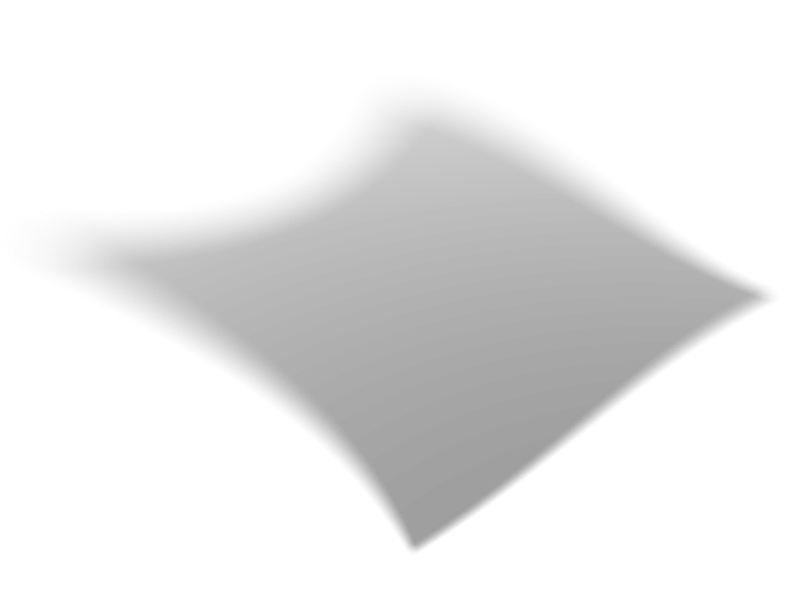
\includegraphics[width=\parampatchimagewidth]{figures/parametric_patch_shadow}};
		}%
		\node[img] at (0,0) {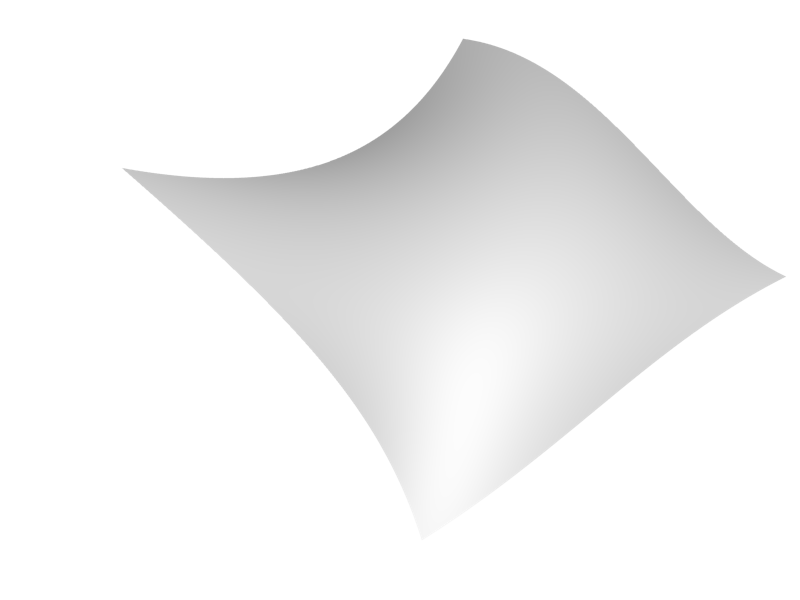
\includegraphics[width=\parampatchimagewidth]{figures/parametric_patch_surface}};
		{\transparent{0.05}%
			\node[img] at (0,0) 	{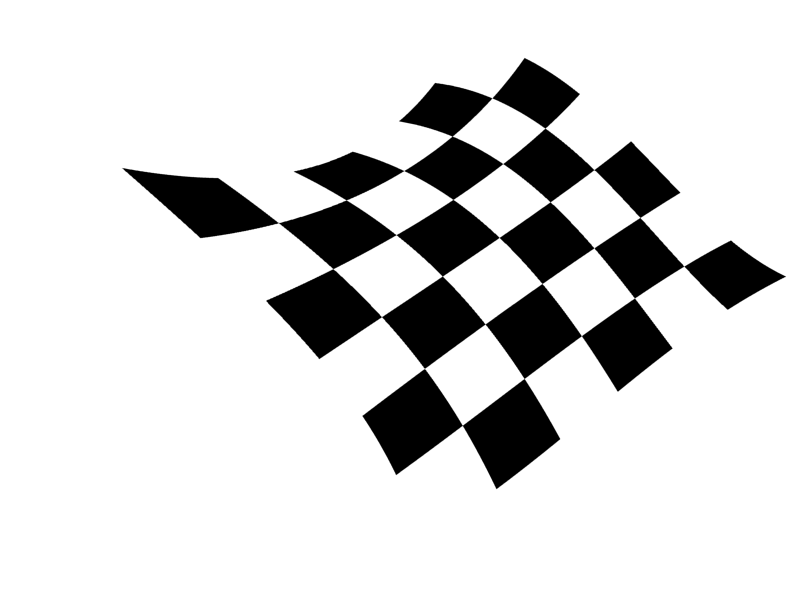
\includegraphics[width=\parampatchimagewidth]{figures/parametric_patch_checkerboard6}};
		}%
		\node[img] at (0,0) {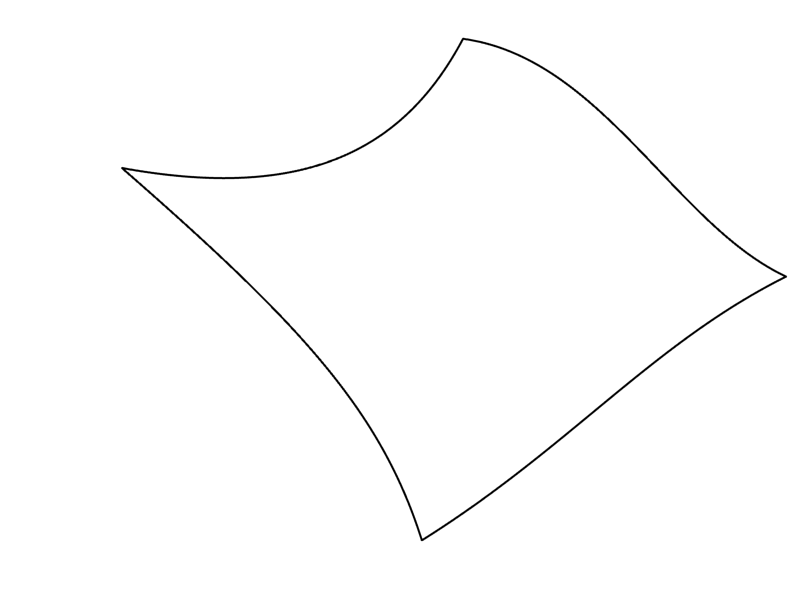
\includegraphics[width=\parampatchimagewidth]{figures/parametric_patch_border}};
		% vecteurs
		\def\scalevectors{1}
		\DTLassign{dbpointonsurf}{2}{\sxco=x,\syco=y}% 
		\DTLassign{dbpointonsurf}{4}{\suxco=x,\suyco=y}% 
		\DTLassign{dbpointonsurf}{5}{\svxco=x,\svyco=y}% 
		\DTLassign{dbpointonsurf}{6}{\nxco=x,\nyco=y}% 
		\DTLassign{dbpointonsurf}{7}{\dsxco=x,\dsyco=y}% 
		\coordinate (s) at (\sxco,\syco);
		\coordinate (su) at (\suxco,\suyco);
		\coordinate (sv) at (\svxco,\svyco);
		\coordinate (n) at (\nxco,\nyco);
		\coordinate (ds) at (\dsxco,\dsyco);
		\draw[dash pattern = on 2pt off 2pt] 
			(su) -- (ds)
			(sv) -- (ds);
		\draw[vector, ducolor] (s) -- (su);% node[label, anchor=north west] {$\bsu$};
		\draw[vector, dvcolor] (s) -- (sv);% node[label, anchor=south] {$\bsv$};
		\draw[vector, black] (s) -- (n) node[label, anchor=south] {$\unv$};
		\draw[vector, dscolor] (s) -- (ds) node[label, anchor=west] {$\dx{\bs}$};
		\fill[black] (s) circle (1.5pt);
		\node [label, anchor=east] at (s) {$\bs(\bu)$};
		%
		\draw[curv] plot file {figures/data/fig_diffgeom_xyzcurve.dat}
			node[label, anchor=east] {$\Gamma$};
		\DTLassign{dbpointoncurv}{4}{\gxco=x,\gyco=y}% 
		\DTLassign{dbpointoncurv}{5}{\dgxco=x,\dgyco=y}% 
		\coordinate (g) at (\gxco,\gyco);
		\coordinate (dg) at (\dgxco,\dgyco);
		\draw[vector] (g) -- ($(g)!\scaledpsi!(dg)$) node[label, anchor=south west] {$\bgw$};
		\fill[black] (g) circle (1.5pt);
		\node [label, anchor=south west, inner sep=0] at (g) {$\bg(w)$};
		%
		% trièdre
		\coordinate (o) at (0.7950445413589478 , 0.19190990924835205);
		\coordinate (x) at (0.6856110692024231 , 0.06267590075731277);
		\coordinate (y) at (0.9558377265930176 , 0.05519538000226021);
		\coordinate (z) at (0.822303831577301 , 0.36832109093666077);
		\draw[axe] (o) -- ($(o)!\scaletriedre!(x)$) node[label, anchor=east] {$x$};
		\draw[axe] (o) -- ($(o)!\scaletriedre!(y)$) node[label, anchor=west] {$y$};
		\draw[axe] (o) -- ($(o)!\scaletriedre!(z)$) node[label, anchor=south] {$z$};
	\end{scope}
	%
	%
	% UV-space
	\def\nuvcells{6}
	\pgfmathsetmacro\uvcellsize{2.0/\nuvcells}
	\begin{scope}[shift={(0,0.375)}, x={0.5*\uvsize}, y={0.5*\uvsize}]
		% UV-domain
		\fill[uvbgcolor] (-1,-1) -- (1,-1) -- (1,1) -- (-1,1) -- cycle;
		\foreach \locj in {1,2,...,\nuvcells}{%
			\pgfmathsetmacro\locy{-1.+(\locj-1)*\uvcellsize}
			\foreach \loci in {1,2,...,\nuvcells}{%
				\pgfmathsetmacro\locx{-1.+(\loci-1)*\uvcellsize}
				\pgfmathsetmacro\modij{int(mod(\loci + \locj,2))}
				\ifnum \modij = 0
					\fill[black!5!uvbgcolor] 
						(\locx,\locy) rectangle ++ (\uvcellsize,\uvcellsize);
				\fi
			}%
		}%
		\draw[semithick] (-1,-1) -- (1,-1) -- (1,1) -- (-1,1) -- cycle;
		% Axes
		\coordinate (o) at ({-1-\distanceaxe},{-1-\distanceaxe});
		\draw[axe] (o) -- ++ ({\fracaxeoffset+\distanceaxe+0.5},0) node [label, anchor=north west] {$u$};
		\draw[axe] (o) -- ++ (0,{\fracaxeoffset+\distanceaxe+0.5}) node [label, anchor=south east] {$v$};
		%
		\DTLassign{dbpointonsurf}{1}{\uvxco=x,\uvyco=y}% 
		\DTLassign{dbpointonsurf}{3}{\duvxco=x,\duvyco=y}% 
		\coordinate (uv) at (\uvxco,\uvyco);
		\coordinate (du) at ([shift={(\duvxco,0)}]uv);
		\coordinate (dv) at ([shift={(0,\duvyco)}]uv);
		\coordinate (duv) at ([shift={(\duvxco,\duvyco)}]uv);
		\draw[dash pattern = on 2pt off 2pt] 
			(du) -- (duv)
			(dv) -- (duv);
		\draw[vector, ducolor] (uv) -- (du);% node[label, anchor=north west] {$\dx{u}$};
		\draw[vector, dvcolor] (uv) -- (dv);% node[label, anchor=south] {$\dx{v}$};
		\draw[vector, dscolor] (uv) -- (duv) node[label, anchor=west] {$\dx{\bu}$};
		\fill[black] (uv) circle (1.5pt);
		\node [label, anchor=north, inner sep=4pt] at (uv) {$\bu$};
		%
		\draw[curv] plot file {figures/data/fig_diffgeom_uvcurve.dat}
			node[label, anchor=west] {$\Psi$};
		\DTLassign{dbpointoncurv}{2}{\uvxco=x,\uvyco=y}% 
		\DTLassign{dbpointoncurv}{3}{\duvxco=x,\duvyco=y}% 
		\coordinate (psi) at (\uvxco,\uvyco);
		\draw[vector] (psi) -- ++ 
		({\scaledpsi*\duvxco,\scaledpsi*\duvyco}) 
		node[label, anchor=south, shift={(2pt,4.5pt)}] {$\bpw$};
		\fill[black] (psi) circle (1.5pt);
		\node [label, anchor=north west, inner sep=0] at (psi) {$\bp(w)$};
		%
	\end{scope}
	%
%	\draw [dotted] (current bounding box.south west) rectangle 
%		(current bounding box.north east);
	%
	% Mappings
	\draw [draw=none] (uv) 
		to [bend left=30] 
		coordinate[pos=0.2] (c)
		coordinate[pos=0.7] (d)
		(s);
	\draw [map] (c) 
		to [bend left=20] 
		node [label, anchor=south west] {$\bs$} 
		(d);
\end{tikzpicture}
%\par\hrule
\caption{Carreau de surface paramétrique\ldots}
\end{figure}
\DTLgdeletedb{dbpointonsurf}%
\DTLgdeletedb{dbpointoncurv}%